\documentclass[12pt,a4paper]{article}
\usepackage[T2A]{fontenc}
\usepackage[utf8]{inputenc}
\usepackage[russian]{babel}
\usepackage{amsmath,amssymb,amsthm}
\usepackage{geometry}
\usepackage{hyperref}
\usepackage{microtype}
\usepackage{setspace}
\usepackage{caption}
\usepackage{graphicx}

\geometry{left=25mm, right=25mm, top=25mm, bottom=25mm}

\hypersetup{
  colorlinks=true,
  linkcolor=black,
  urlcolor=blue,
  pdfauthor={Тишковец Сергей},
  pdftitle={Отчёт по курсовой работе — Часть №3}
}

\begin{document}
\selectlanguage{russian}

\begin{titlepage}
  \begin{center}
    {Санкт-Петербургский политехнический университет Петра Великого\\
    Институт прикладной математики и механики\\[0.5em]
    \textbf{Высшая школа прикладной математики и вычислительной физики}}
    
    \vfill
    
    {\LARGE\bfseries Отчёт по курсовой работе\\ Часть №3\par}
    \vspace{1em}
    {\Large по дисциплине\\[0.3em] {\bfseries «Проект по математической статистике»}}
    
    \vfill
    
    \begin{flushright}
        Выполнил\\
        студент гр. 5030102/20202: Тишковец Сергей
    \end{flushright}
    
    \begin{flushright}
        Проверил\\
        Преподаватель: Заяц Олег Иванович
    \end{flushright}
    
    \vfill
    Санкт-Петербург\\
    2026
  \end{center}
\end{titlepage}

\setcounter{page}{2}
\newpage

\section*{Вычисление ОИСКО ОМП: равномерное распределение}

Рассмотрим задачу оценивания плотности равномерного распределения методом максимального правдоподобия. Истинная плотность задана как:
\[
f_0(x) = 
\begin{cases}
\dfrac{1}{2\sqrt{3}}, & |x| \le \sqrt{3}, \\
0, & |x| > \sqrt{3}.
\end{cases}
\]

В общем случае для распределения $U[a, b]$ неизвестными параметрами являются границы интервала. Истинные значения параметров: $a = -\sqrt{3}$, $b = \sqrt{3}$, длина носителя $L = b - a = 2\sqrt{3}$.

Оценками максимального правдоподобия (ОМП) для границ $a$ и $b$ являются крайние порядковые статистики выборки:
\[
\hat{a} = X_{(1)} = \min_{1 \le i \le n} X_i, \quad \hat{b} = X_{(n)} = \max_{1 \le i \le n} X_i.
\]

Оценка плотности вероятности методом максимального правдоподобия имеет вид:
\[
\hat{f}(x) = 
\begin{cases}
\dfrac{1}{\hat{L}}, & x \in [\hat{a}, \hat{b}], \\
0, & x \notin [\hat{a}, \hat{b}],
\end{cases}
\]
где $\hat{L} = \hat{b} - \hat{a}$ — размах выборки. Поскольку $\hat{a} \ge a$ и $\hat{b} \le b$ почти наверное, интервал $[\hat{a}, \hat{b}]$ вложен в $[a, b]$. 

Интегральная среднеквадратическая ошибка (ISE) принимает вид:
\[
\text{ISE} = \int_{-\infty}^{\infty} (\hat{f}(x) - f_0(x))^2 \,dx = \int_{\hat{a}}^{\hat{b}} \left(\frac{1}{\hat{L}} - \frac{1}{L}\right)^2 \,dx + \int_{a}^{\hat{a}} \left(\frac{1}{L}\right)^2 \,dx + \int_{\hat{b}}^{b} \left(\frac{1}{L}\right)^2 \,dx.
\]
После алгебраических преобразований интеграл сводится к:
\[
\text{ISE} = \hat{L} \frac{(L - \hat{L})^2}{L^2 \hat{L}^2} + \frac{\hat{a} - a}{L^2} + \frac{b - \hat{b}}{L^2} = \frac{(L - \hat{L})^2}{L^2 \hat{L}} + \frac{L - \hat{L}}{L^2} = \frac{L - \hat{L}}{L \hat{L}} = \frac{1}{\hat{L}} - \frac{1}{L}.
\]

Для вычисления математического ожидания $\mathbb{E}[1/\hat{L}]$ воспользуемся тем, что случайная величина $\hat{L}/L$ распределена как размах выборки из стандартного равномерного распределения $U[0, 1]$. Плотность размаха $V = \hat{L}/L$ равна $f_V(v) = n(n-1)v^{n-2}(1-v)$ для $v \in [0,1]$.
\[
\mathbb{E}\left[\frac{1}{\hat{L}}\right] = \frac{1}{L} \mathbb{E}\left[\frac{1}{V}\right] = \frac{n(n-1)}{L} \int_0^1 v^{n-3}(1-v) \,dv = \frac{n}{L(n-2)}.
\]

Тогда математическое ожидание ISE равно:
\[
\text{MISE} = \mathbb{E}[\text{ISE}] = \frac{n}{L(n-2)} - \frac{1}{L} = \frac{2}{L(n-2)}.
\]

Относительное интегральное среднеквадратическое отклонение (ОИСКО):
\[
\bar{\delta}_n = \frac{\text{MISE}}{\int_{-\infty}^{\infty} f_0^2(x)\,dx}.
\]
Поскольку $\int f_0^2(x)\,dx = 1/L$, итоговая аналитическая формула ОИСКО для ОМП имеет вид:
\[
\bar{\delta}_n = \frac{2}{n - 2}.
\]

\section*{Построение графиков}

\subsection*{График 1. Зависимость нижней границы погрешности $\bar{\delta}_{n,\min}$ от $n$}
\begin{figure}[ht!]
    \centering
    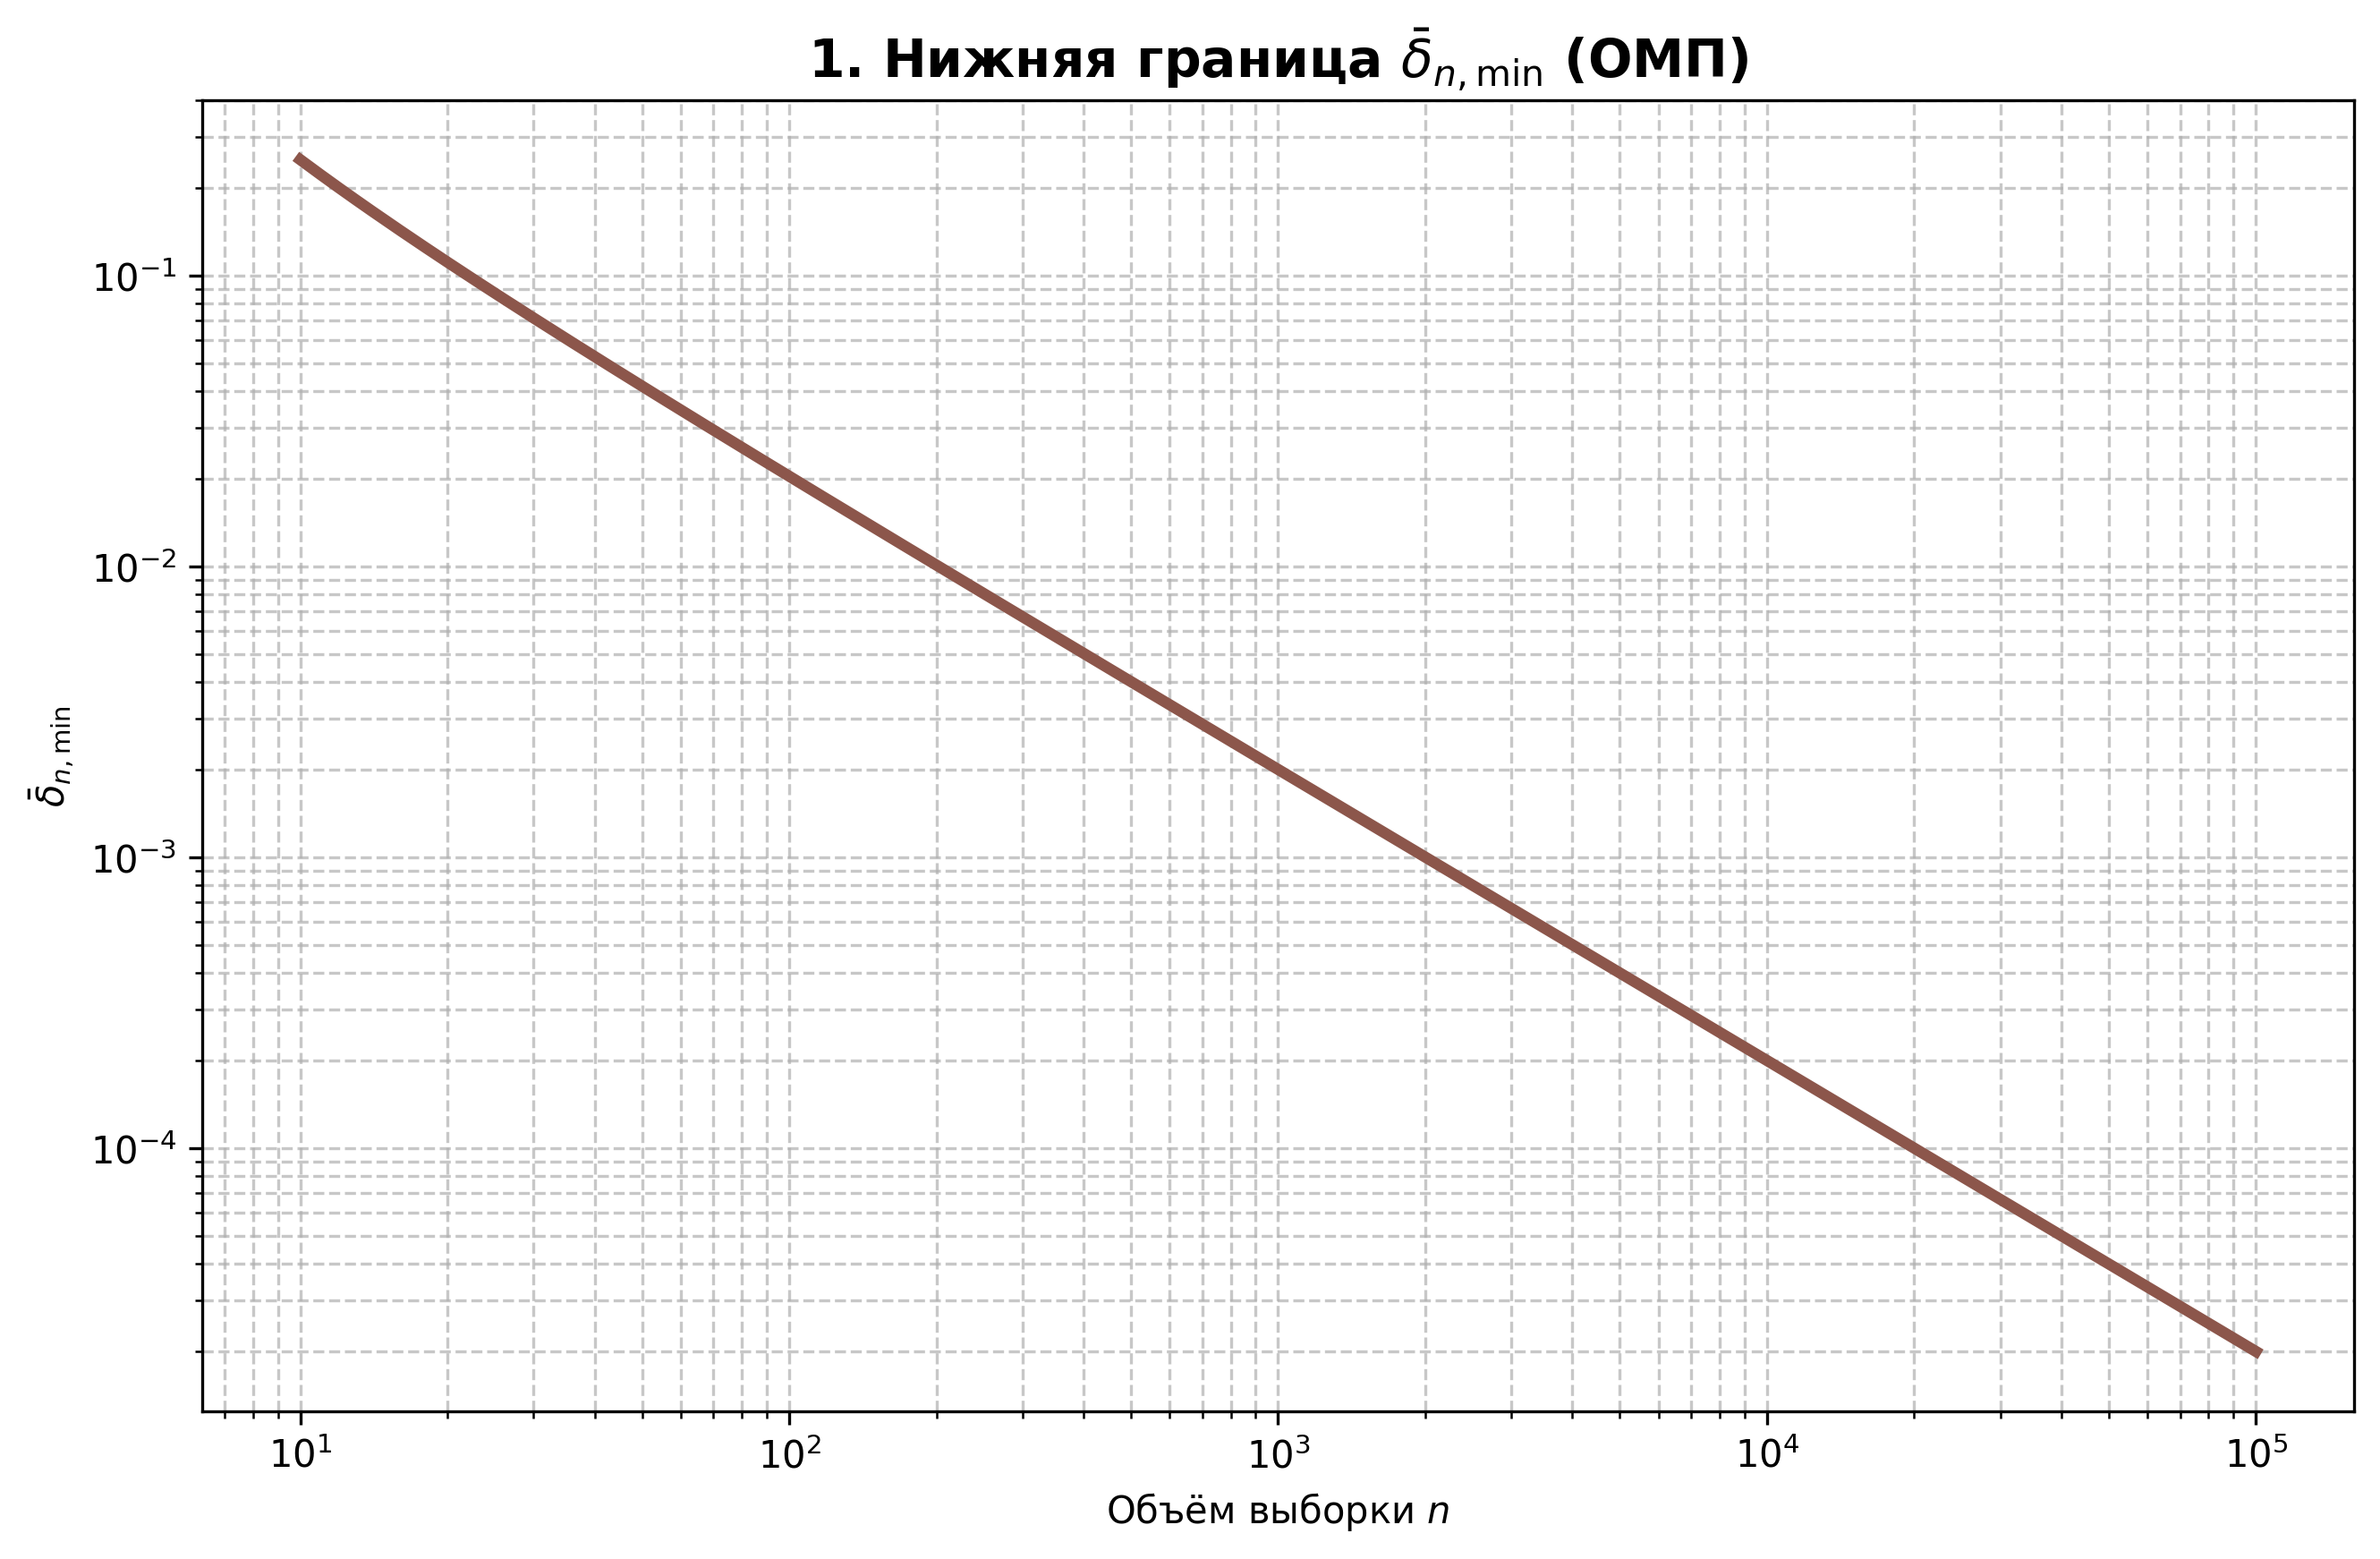
\includegraphics[width=0.85\textwidth]{figures/f9.png}
    \caption{Минимальное ОИСКО ОМП (в логарифмическом масштабе)}
    \label{fig:omp_delta_min}
\end{figure}

\subsection*{График 2. Сравнение Ядерной оценки (ЯО) и ОМП}
\begin{figure}[ht!]
    \centering
    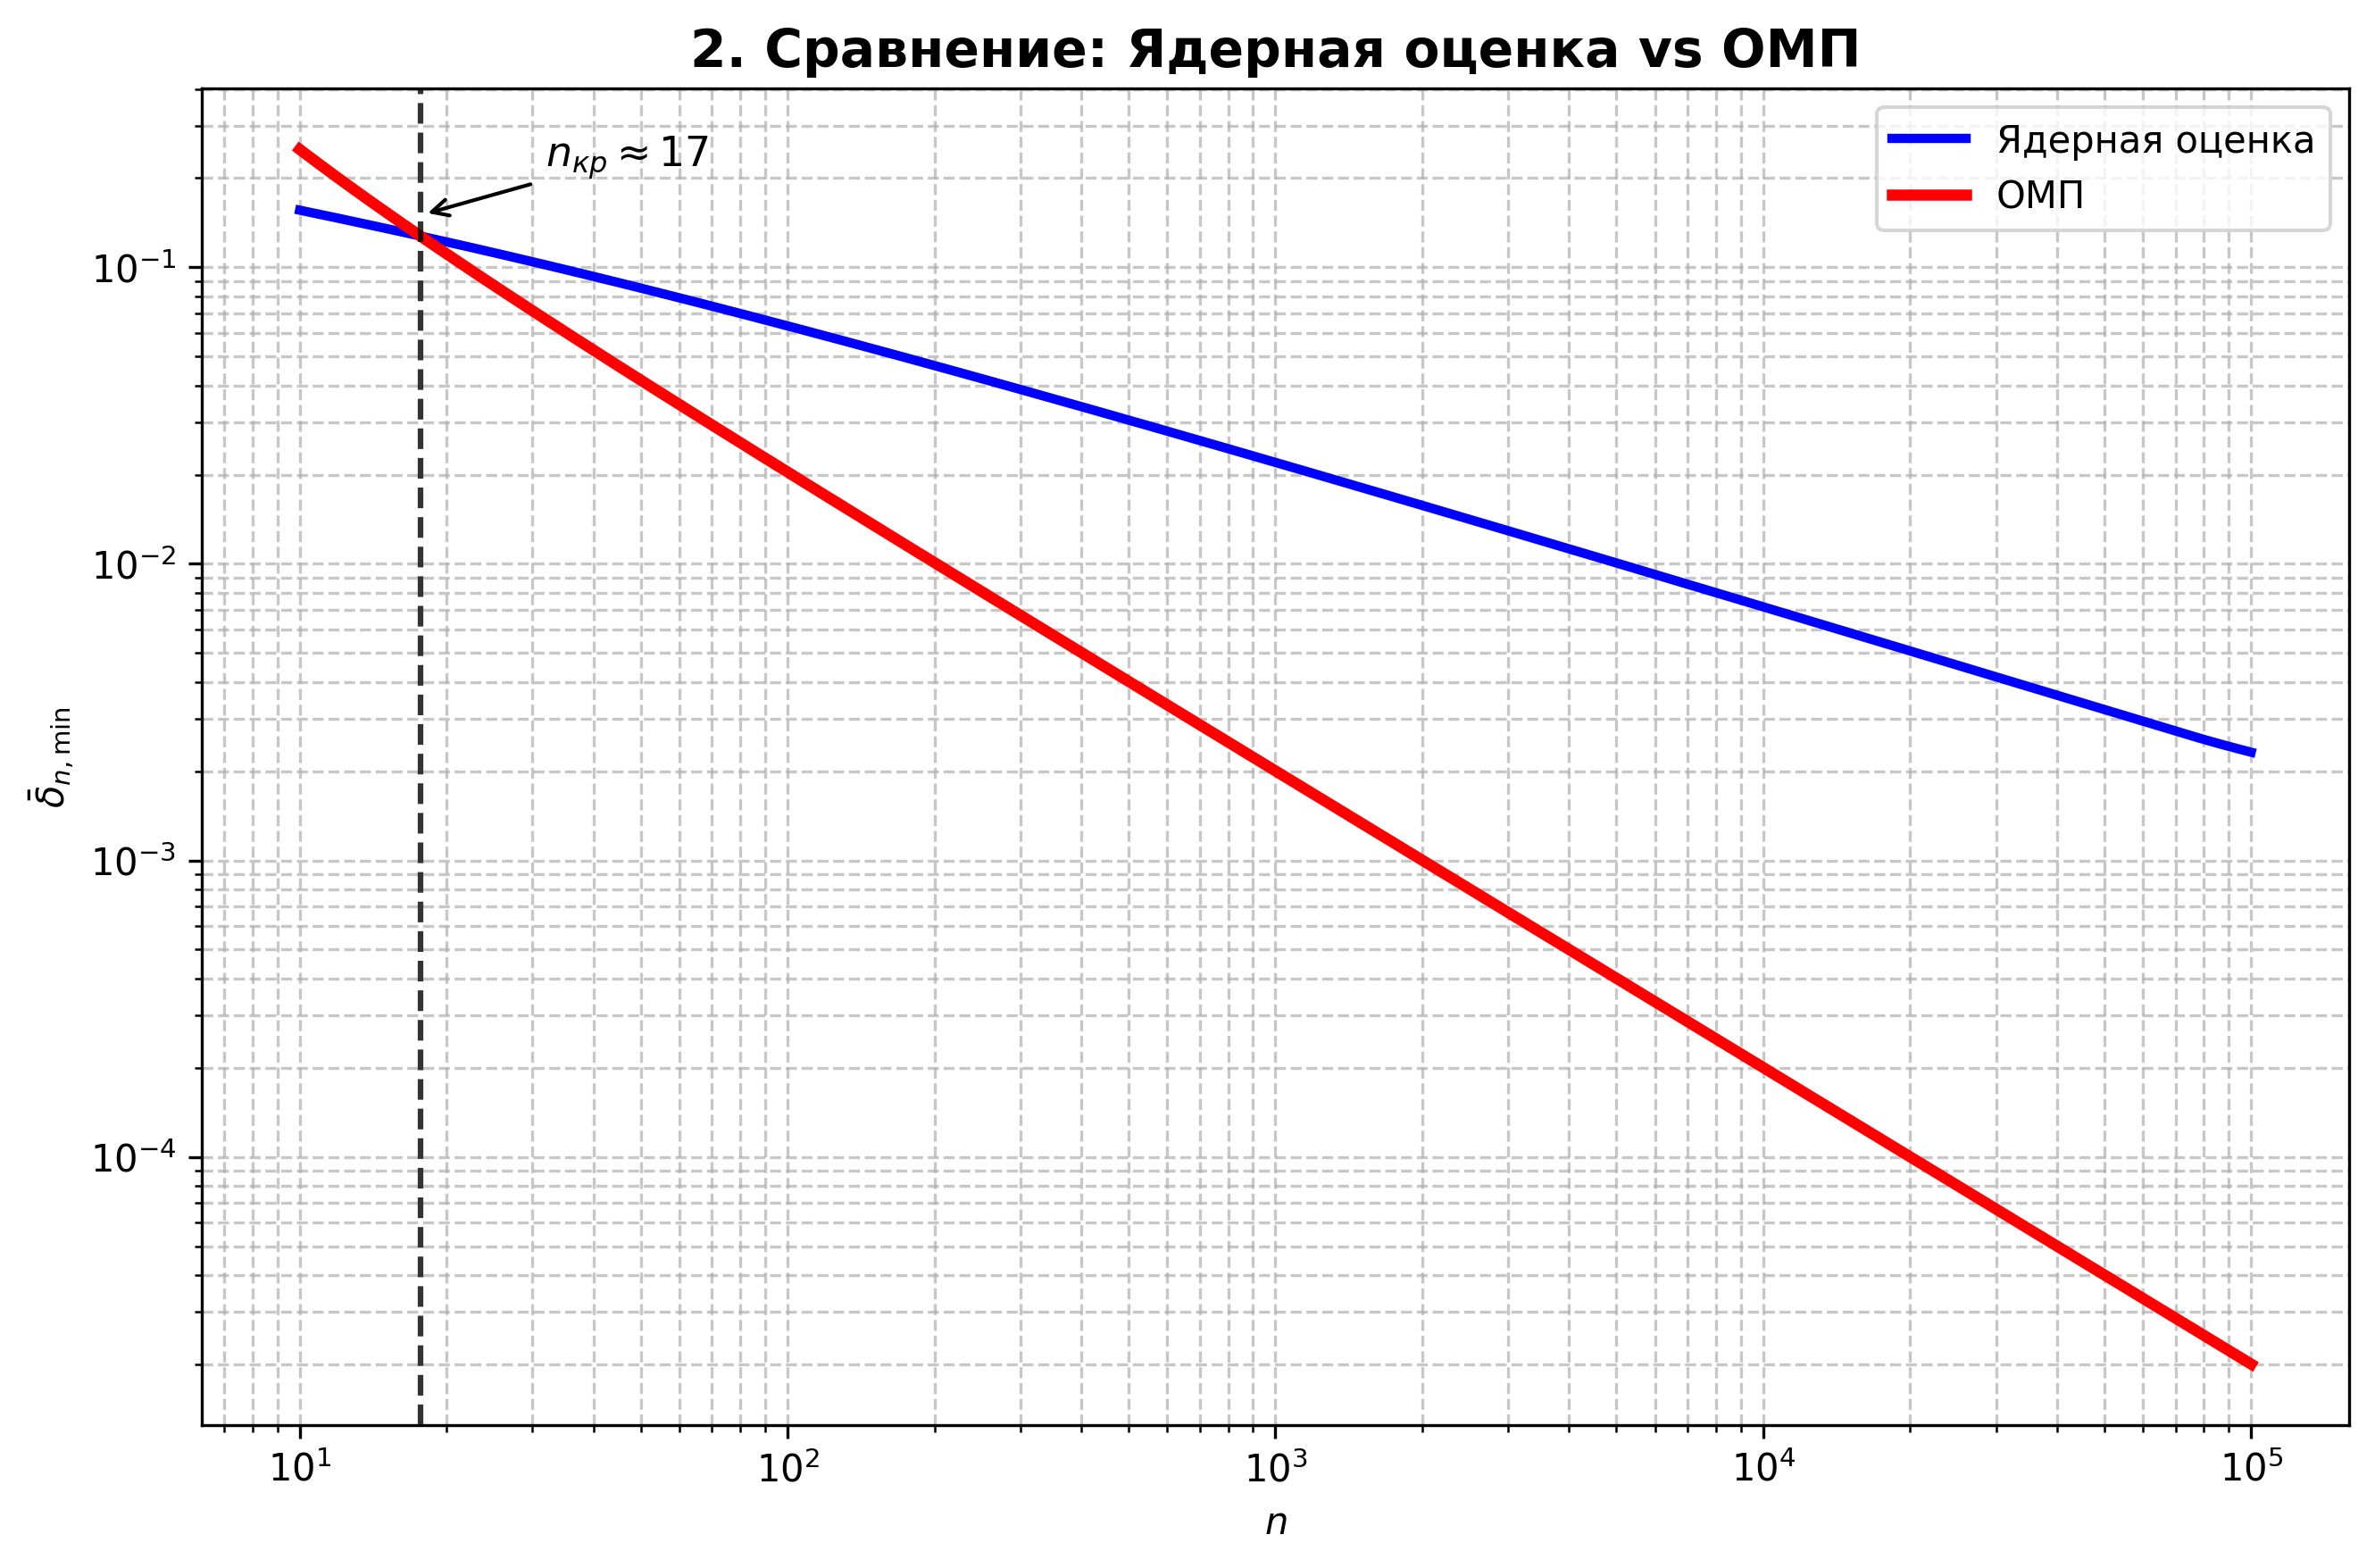
\includegraphics[width=0.85\textwidth]{figures/f10.png}
    \caption{Сравнение ОИСКО ЯО и ОМП (в логарифмическом масштабе)}
    \label{fig:comparison_kde}
\end{figure}

\subsection*{График 3. Сравнение Гистограммы и ОМП}
\begin{figure}[ht!]
    \centering
    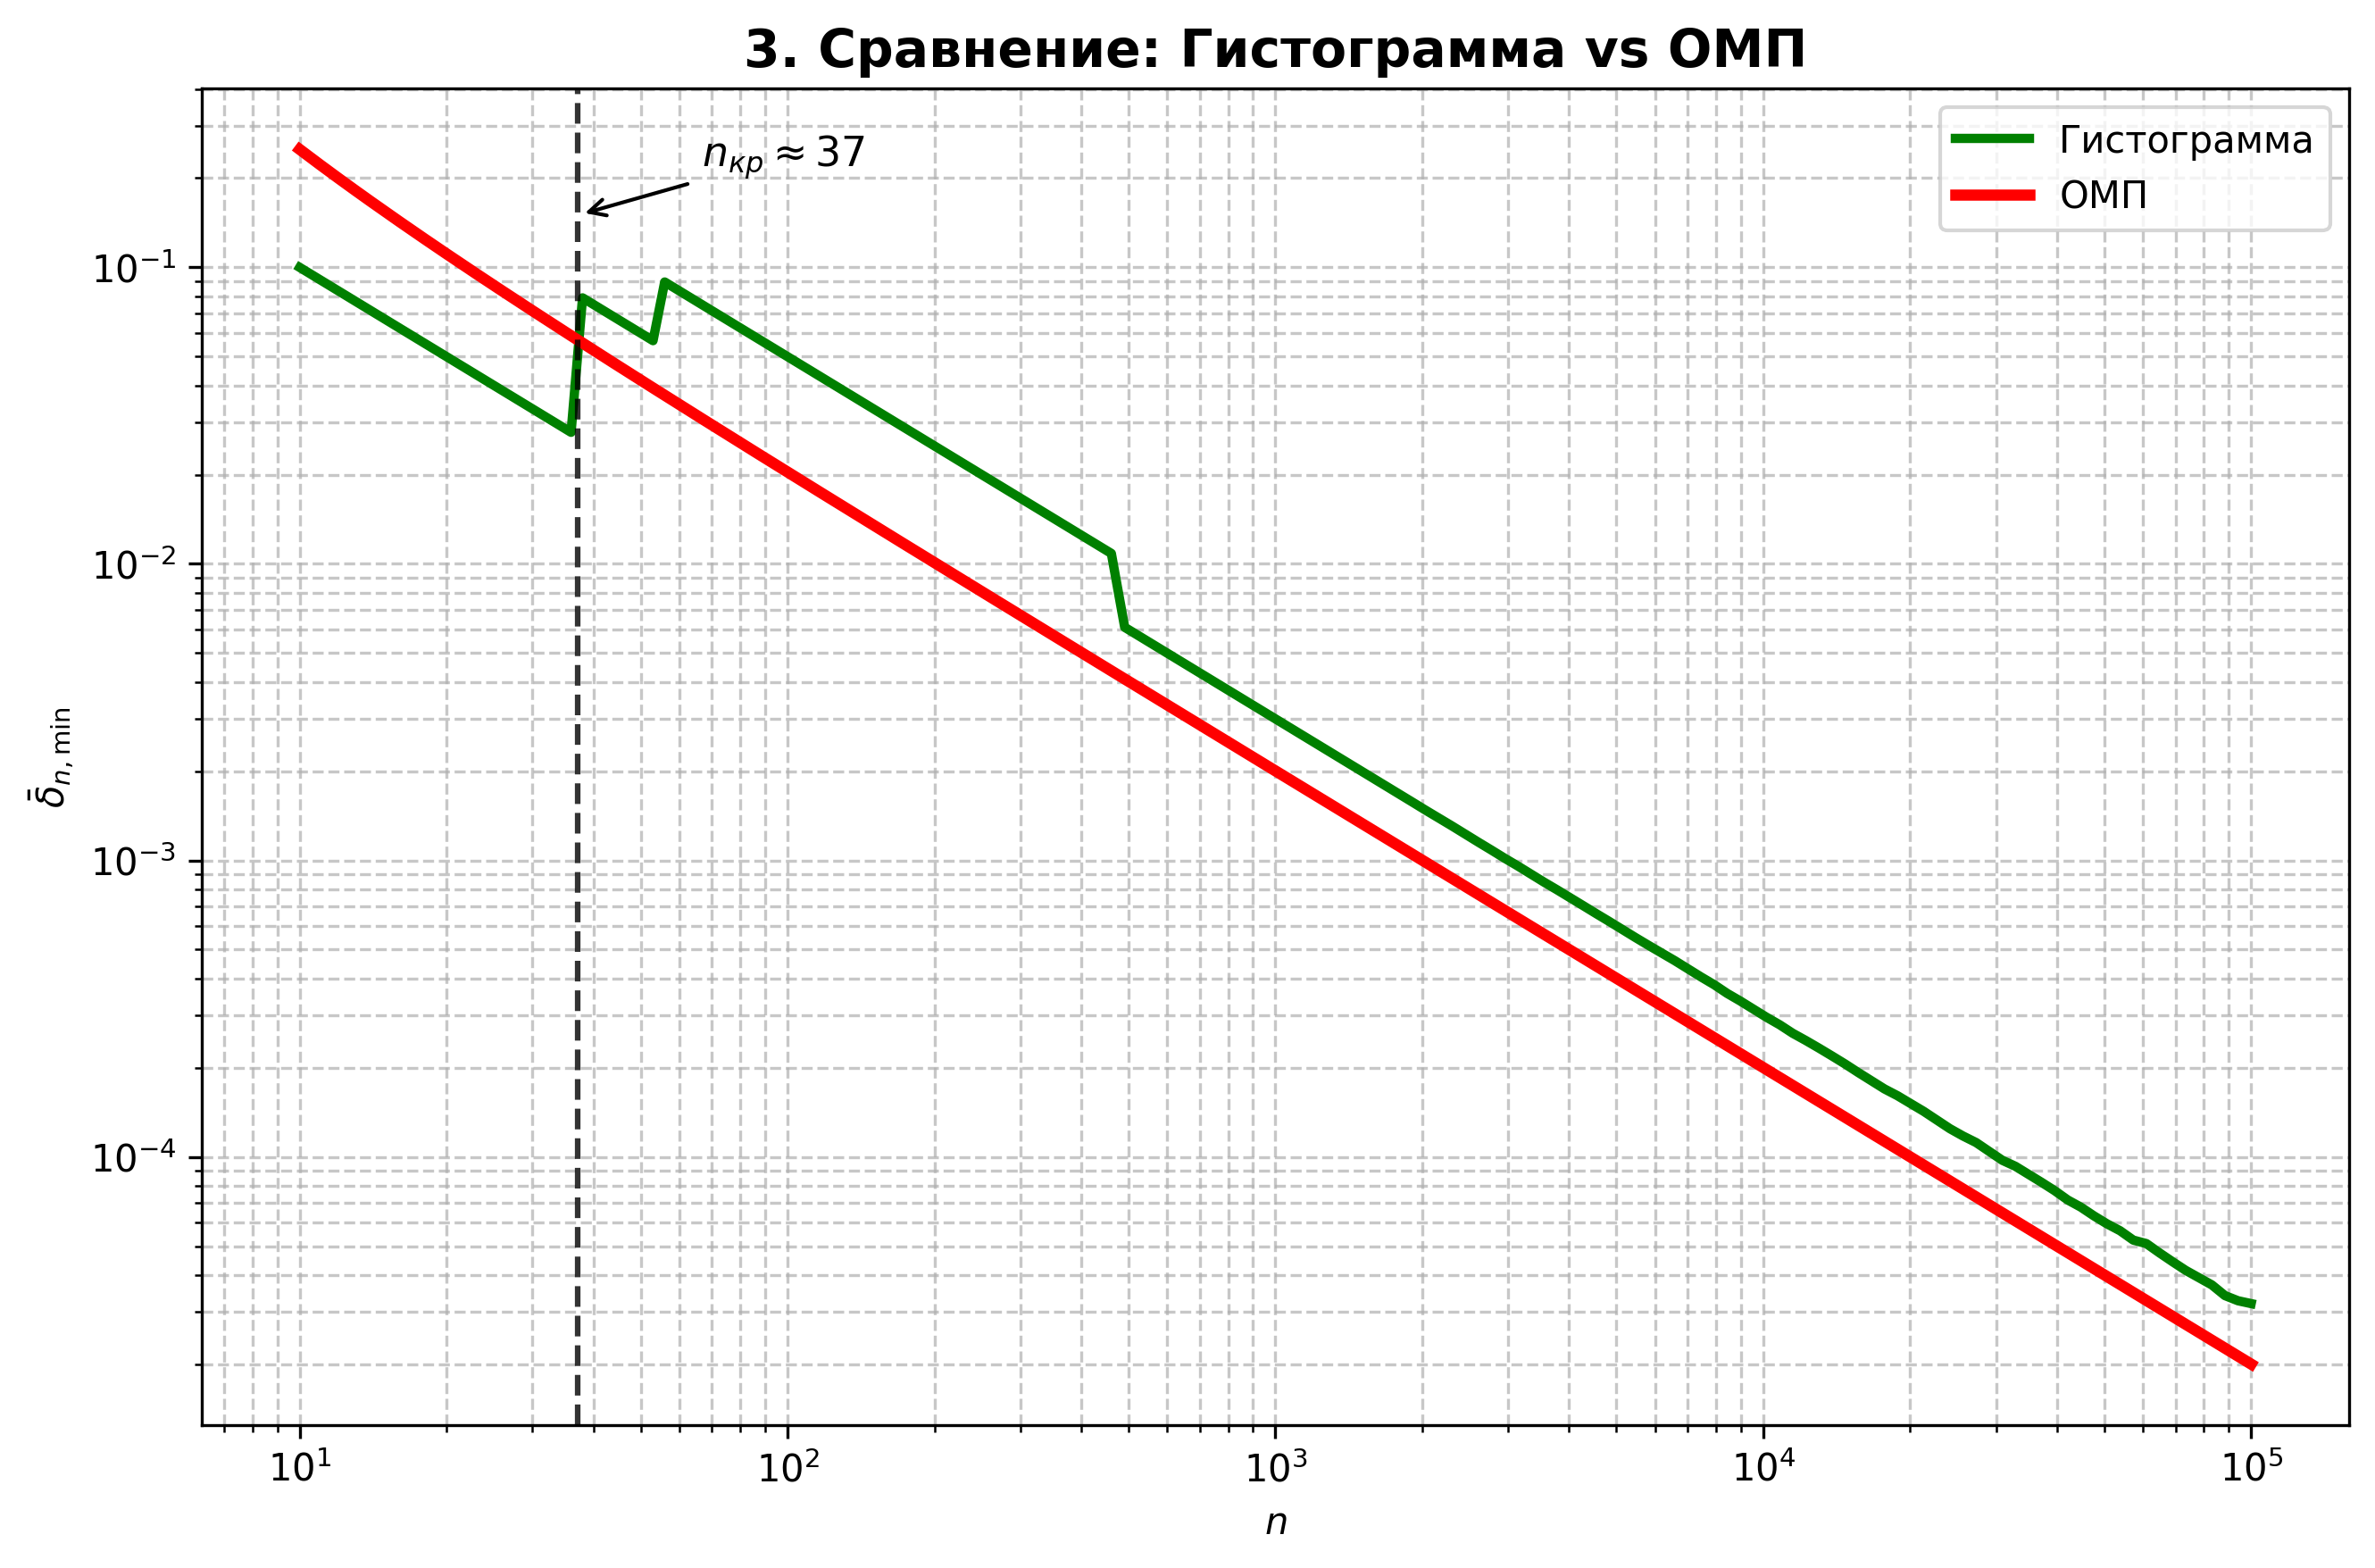
\includegraphics[width=0.85\textwidth]{figures/f11.png}
    \caption{Сравнение ОИСКО Гистограммы и ОМП (в логарифмическом масштабе)}
    \label{fig:comparison_hist}
\end{figure}

\newpage
\section*{Выводы}

В рамках курсовой работы были исследованы три метода оценивания плотности равномерного распределения: 
ядерная оценка (с колокольным ядром), гистограммная оценка и оценка максимального правдоподобия (ОМП). 
Сравнение проводилось по критерию относительного интегрального среднеквадратического отклонения (\(\bar{\delta}_n\)).

Теоретически известно, что ОМП обладает параметрической скоростью сходимости \(O(1/n)\), 
тогда как ядерная оценка имеет скорость \(O(n^{-4/5})\), а гистограмма — \(O(n^{-2/3})\). 
Это задаёт ожидаемое асимптотическое преимущество ОМП при больших объёмах выборки.

По результатам численных экспериментов получены следующие критические значения:

\begin{itemize}
    \item \(n_{\text{кр}} \approx 17\) — для пары «ядерная оценка -- ОМП»;
    \item \(n_{\text{кр}} \approx 37\) — для пары «гистограмма -- ОМП»;
    \item \(n_{\text{кр}} \approx 17\) — для пары «ядерная оценка -- гистограмма».
\end{itemize}

На основании этих значений можно выделить три характерные области:

\begin{itemize}
    \item \textbf{Малые выборки (\(n \lesssim 17\)).}  
    Наилучшие результаты демонстрирует ядерная оценка.

    \item \textbf{Средние выборки (\(17 \lesssim n \lesssim 37\)).}  
    Наиболее точной становится гистограммная оценка. В этом диапазоне она превосходит как ядерную оценку, так и ОМП по значению ОИСКО.

    \item \textbf{Большие выборки (\(n \gtrsim 37\)).}  
    Наименьшее значение ошибки достигается оценкой максимального правдоподобия. Это согласуется с её более быстрой асимптотической скоростью сходимости.
\end{itemize}

Таким образом, оптимальный выбор метода зависит от \(n\): 
ядерная оценка предпочтительна на малых выборках, гистограмма — на промежуточных, 
а ОМП — на больших.

\end{document}